\newsavebox{\smlmat}
\savebox{\smlmat}{$\smm{\bullet&\bullet\\\bullet& }$}
\newsavebox{\smlmatb}
\savebox{\smlmatb}{$\smm{\bullet&\bullet\\\bullet&\bullet}$}
\newsavebox{\smlmatc}
\savebox{\smlmatc}{$\smm{\bullet&\bullet&\bullet\\ &\bullet& }$}

\chapter{Small interval minors}
\label{chap:chars}
Our goal in this chapter is to describe, for a given small pattern, the structure of matrices avoiding it as an interval minor.

Algorithmically speaking, deciding whether a pattern is contained in a matrix is NP-hard, even if both matrices are permutation matrices, see \cite{complex}. We do not consider complexity questions here, but for small patterns, we show that matrices avoiding them have a quite simple structure. However, the structure gets significantly more complex as soon as we allow the pattern to contain at least four one-entries.

To go through cases efficiently, we first show that to some extent, we can assume, without loss of generality, there are no empty lines in studied patterns.

Before we dive into characterizations, let us introduce some useful notion.

\begin{defn}
A \emph{walk} in a matrix~$M$ is a contiguous sequence of its entries, beginning in the top-left corner and ending in the bottom-right one. If $M[i,j]$ occurs in the sequence, its successor is either $M[i+1,j]$ or $M[i,j+1]$. Symmetrically, a \emph{reverse walk} in $M$ is a contiguous sequence of its entries, beginning in the top-right corner and ending in the bottom-left one.
\end{defn}

\begin{defn}
We say a matrix~$M$ is a \emph{walking matrix} if there is a walk in $M$ containing all one-entries.
\end{defn}

\begin{defn}
For a matrix~$M\in\Mat$ and integers $r,c$, we say $M[r,c]$ is
\begin{itemize}
	\item \emph{top-left empty}, if $M[[r-1],[c-1]]$ is an empty matrix,
	\item \emph{top-right empty}, if $M[[r-1],[c+1,n]]$ is empty,
	\item \emph{bottom-left empty}, if $M[[r+1,m],[c-1]]$ is empty,
	\item \emph{bottom-right empty}, if $M[[r+1,m],[c+1,n]]$ is empty.
\end{itemize}
\end{defn}

\begin{defn}
For a matrix~$M\in\Mat$ and integers $r,c$, we say that an entry~$M[r,c]$ is \emph{top-left extreme}, if it is top-left empty and the submatrix~$M[[r],[c]]$ is not empty. Similarly, $M[r,c]$ is \emph{bottom-right extreme} if it is bottom-right empty and the submatrix~$M[[r,m],[c,n]]$ is not empty. A walk in $M$ is \emph{top-left extreme} if it contains all top-left extreme elements of $M$. A reverse walk in $M$ is \emph{bottom-right extreme} if it contains all bottom-right extreme elements of $M$.
\end{defn}

It is easy to see that there is exactly one bottom-left extreme walk and exactly one bottom-right extreme walk in every non-empty matrix.

\begin{defn}
For matrices $M\in\Mat$ and $N\in\bin^{m\times l}$, we define $M\hsum N\in\bin^{m\times(n+l)}$ to be the matrix created from $M$ by appending the columns of~$N$ at the end of $M$.
\end{defn}

\section{Empty rows and columns}
\label{sec:empty}
From the definition of matrix containment, zero-entries of the pattern pose no restrictions on the tested matrix, so, intuitively, adding new empty lines to a pattern should not influence the structure of matrices avoiding the pattern by much.

We first show that adding empty lines as first or last lines of the pattern indeed does next to no difference. On the other hand, inserting empty lines in between non-empty lines becomes a bit more tricky and we only describe what happens when we extend a pattern of size $k\times2$ (or symmetrically $2\times k$) by a single empty column (row).

\begin{obs}
\label{obs:emptyrows}
For matrices~$P\in\Pat$ and $M\in\Mat$, let $P'=P\hsum\{0\}^{k\times1}$ and let $M'=M\hsum\{1\}^{m\times1}$. Then $\PimM\Leftrightarrow P'\im M'$.
\end{obs}
\begin{proof}
\begin{itemize}
	\item[$\Rightarrow$] The last column of $P'$ can always be mapped just to the last column of $M'$ and $P'[[k],[l]]$ can be mapped to $M'[[m],[n]]$ the same way $P$ is mapped to $M$.
	\item[$\Leftarrow$] Taking the restriction of the mapping of $P'$ to $M'$, we get a mapping of $P$ to $M$. \qedhere
\end{itemize}
\end{proof}

The analogous proof can be also used to characterize matrices avoiding patterns after adding an empty column as the first column or an empty row as the first or the last row. Using induction, we can easily show that a pattern $P'$ is avoided by a matrix $M'$ if and only if $P$ is avoided by $M$, where $P$ is derived from $P'$ by excluding all empty leading or ending rows and columns and $M$ is derived from $M'$ by excluding the same number of leading or ending rows and columns. Therefore, when characterizing matrices avoiding a forbidden pattern, we do not need to consider patterns having empty rows or columns on their boundary.

We now show what happens when we add an empty column in between two columns of a pattern that only has two columns. It is going to be achieved by employing a notion of intervals of one-entries. More about these intervals and their counterpart -- zero-intervals can be found in the last chapter of the thesis.

\begin{defn}
A \emph{one-interval} of a matrix~$M$ is a sequence of consecutive one-entries of a single line of $M$ bounded from each side by a zero-entry or the edge of the matrix.
\end{defn}

\begin{defn}
For a class of matrices~$\class{M}$, a matrix~$M\in\class{M}$ is \emph{critical} in $\class{M}$ if after a change of any zero-entry to one-entry the matrix no longer belongs to $\class{M}$. For a pattern~$P$, we denote by $\Avmax{P}$ the set of all matrices critical in $\Avm{P}$. 
\end{defn}

\begin{lemma}
\label{lemma:twocols}
For every $l>1$, let $P\in\bin^{k\times l}$ be a pattern such that only the first and the last columns are non-empty and let $M\in\Avmax{P}$ be a matrix, then $M$ contains at most one one-interval in each row.
\end{lemma}
\begin{proof}
For contradiction, assume there are at least two one-intervals in a row of $M$. Because $M$ is critical in $\Avm{P}$, changing any zero-entry~$e$ in between one-intervals $o_1$ and $o_2$ creates a mapping of the forbidden pattern. Such a mapping uses the changed one-entry to map some element $P[r',1]$ or $P[r',l]$.

In the first case, the same mapping also maps $P$ to $M$ if we use a one-entry from $o_1$ instead of $e$; thus, $\PimM$ and we reach a contradiction. In the second case, the mapping can use a one-entry from $o_2$ instead of $e$; therefore, we again get a contradiction with $\PnimM$. Since $e$ is not usable for any one-entry of $P$, we can change it to a one-entry and get a contradiction with $M$ being critical.
\end{proof}

\begin{lemma}
\label{lemma:maxmult}
Let $P\in\bin^{k\times3}$ be a pattern such that its middle column is empty. Every row of any matrix~$M\in\Avmax{P}$ is either empty or it contains a single one-interval of length at least $2$ (or length $m$ if $m<2$).
\end{lemma}
\begin{proof}
Let a matrix~$M\in\Avmax{P}$. The same proof as in Lemma~\ref{lemma:twocols} shows that there is at most one one-interval in each row of $M$. For contradiction, let there be only one one-entry~$M[r,c]$ in a row~$r$:
\begin{itemize}
	\item $c=1$: we can set $M[r,c+1]=1$ and the matrix still avoids $P$, which is a contradiction with $M$ being critical in $\Avm{P}$.
	\item $c=n$: we can set $M[r,c-1]=1$ and the matrix still avoids $P$, which is a contradiction with $M$ being critical in $\Avm{P}$.
	\item otherwise: consider zero-entries $e_l=M[r,c-1]$ and $e_r=M[r,c+1]$. For contradiction, assume we can change neither $e_l$ nor $e_r$ to a one-entry without creating a mapping of the pattern. It means that if we set $e_l=1$ then some $P[r_1,1]$ can be mapped to it. Let $m_l$ be the corresponding mapping. At the same time, if we set $e_r=1$ then some $P[r_2,3]$ can be mapped to it and $m_r$ is the corresponding mapping. We show that the two mappings can be combined to a mapping of $P$ to $M$, giving a contradiction.
	
	Without loss of generality, in both mappings, the empty column of $P$ is mapped exactly to the column~$c$ of $M$. We need to describe how to partition $M$ into $k$ rows. Consider Figure~\ref{fig:emptymid}:
	\begin{itemize}
		\item $r_1\neq r_2$: Without loss of generality, we assume $r_1>r_2$. Let $r_3$ be the first row of the interval where the row~$r_1$ is mapped in $m_l$ and let $r_4$ be the last row of the interval where the row~$r_1$ is mapped in $m_r$. From the mapping~$m_l$, we know that the first $r_1-1$ rows of $P$ can be mapped to rows $[1,r_3-1]$ and from the mapping~$m_r$, we know that the last $k-r_1$ rows of $P$ can be mapped to rows $[r_4+1,m]$. From the mapping~$m_r$, we know that the row~$r_1$ can be mapped to rows $[r_3,r_4]$; thus, we have a mapping of $P$ to $M$.
		\item $r_1=r_2$: Let $[r_3,r_4]$ be the interval where the row~$r_1$ is mapped in $m_l$ and let $[r_5,r_6]$ be the interval where the row~$r_1$ is mapped in $m_r$. Without loss of generality, let $r_3<r_5$. From the mapping~$m_l$, we know that the first $r_1-1$ rows of $P$ can be mapped to rows $[1,r_3-1]$. Without loss of generality, let $r_4<r_6$. From the mapping~$m_r$, we know that the last $k-r_1$ rows of $P$ can be mapped to rows $[r_6+1,m]$. Therefore, we can map the row~$r_1$ of $P$ to the row interval~$[r_3,r_6]$ without using one-entries $e_l$ and $e_r$.
	\end{itemize}
\end{itemize}
We showed that either $e_l$ or $e_r$ can be changed to a one-entry, which is a contradiction with $M$ being critical in $\Avm{P}$.
\end{proof}

\begin{figure}[!ht]
\centering
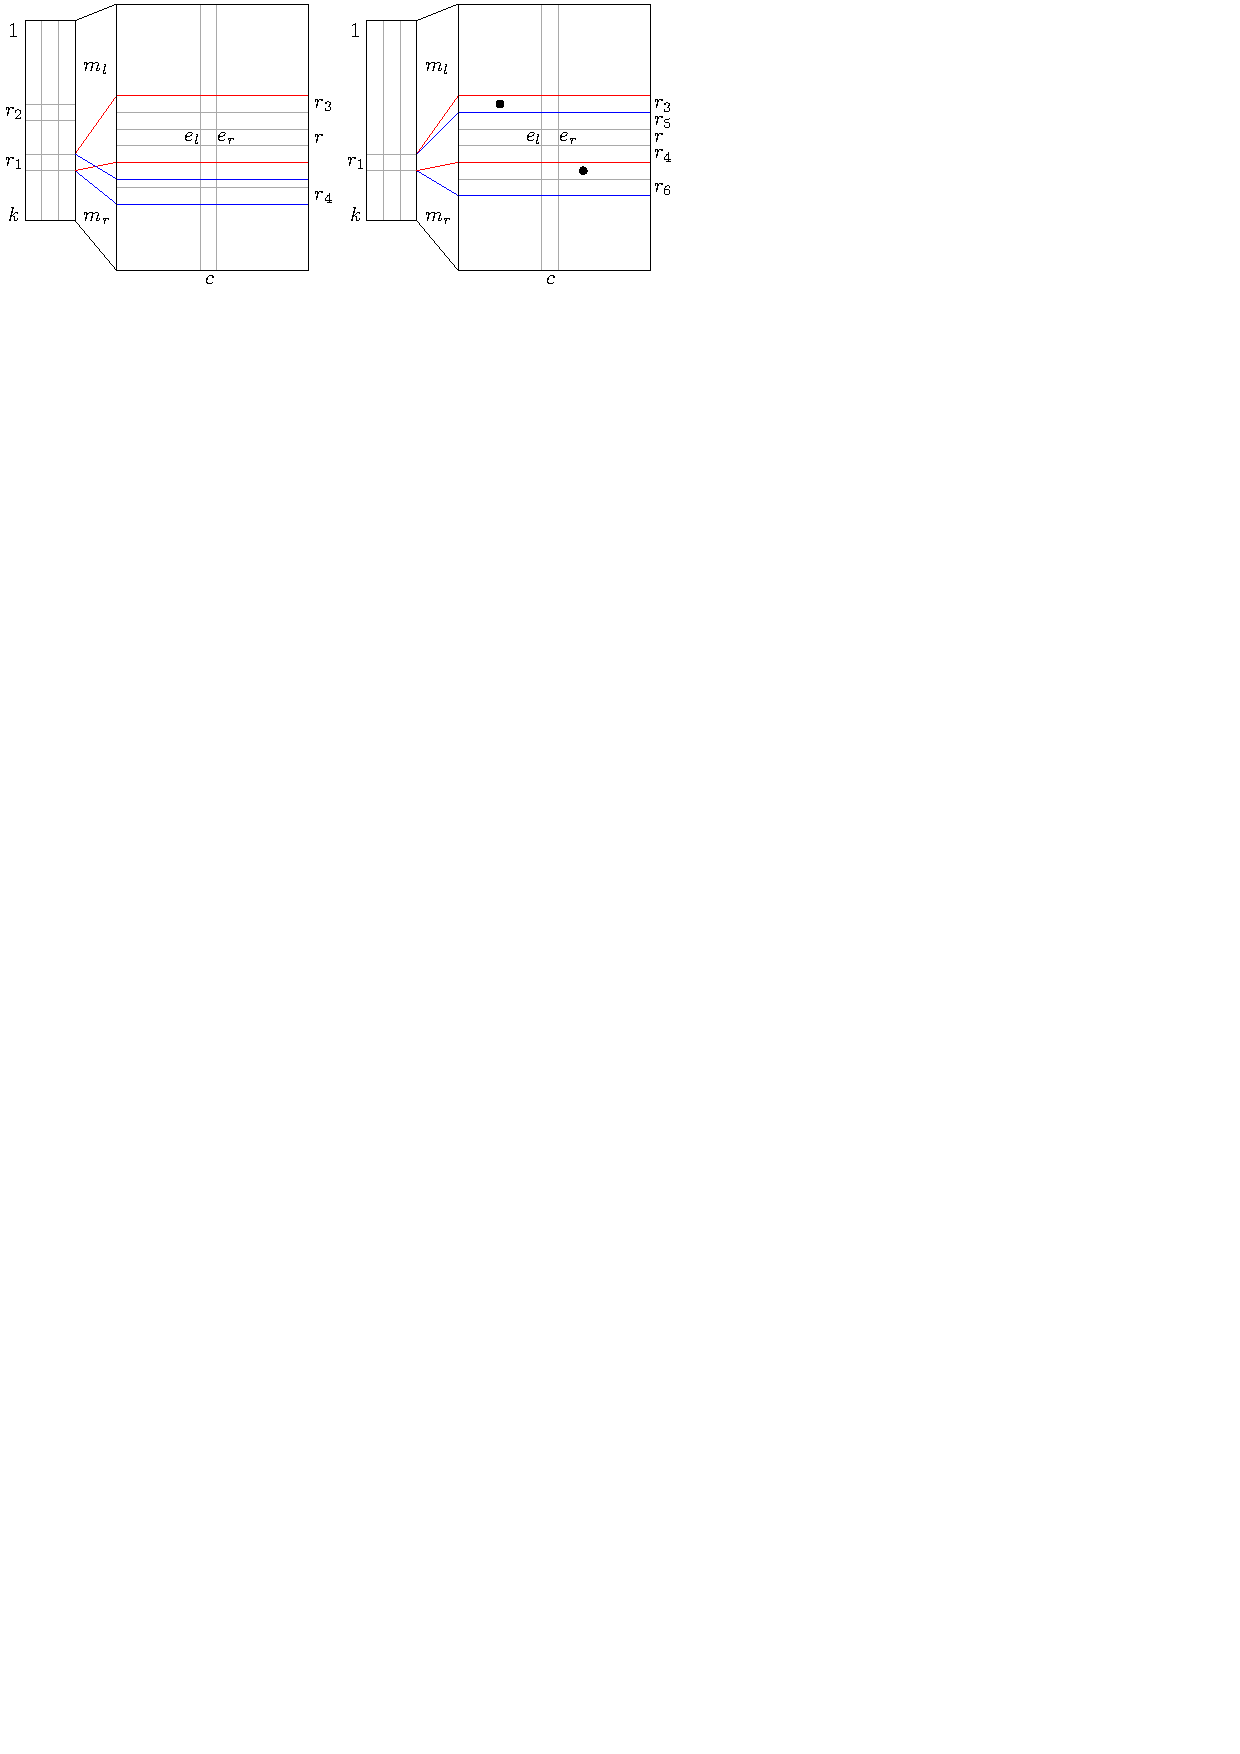
\includegraphics[width=130mm]{img/emptymidcol.pdf}
\caption{Red and blue lines representing mappings $m_l$ and $m_r$ of the forbidden pattern. The two horizontal lines show the boundaries of the mapping of the row~$r$ and the vertical lines show the boundaries of the mapping of the column~$c$.}
\label{fig:emptymid}
\end{figure}

Similarly, we can prove that for every pattern~$P\in\Pat$ such that all $(l-2)$ middle columns are empty, every matrix from $\Avmax{P}$ that contains at least $l$ one-entries in each row, contains at least $l+1$ one-entries in each row. On the other hand, it cannot be generalized further, as we show in the following proposition.

\begin{prop}
For every integer $l>3$, there exists a pattern~$P\in\Pat$ such that all $(l-2)$ middle columns are empty and there exists a matrix~$M\in\Avmax{P}$ containing a row with a single one-entry.
\end{prop}
\begin{proof}
We only show the construction for $l=4$ and $l=5$ because the first construction can easily be extended for every even $l$ and the latter for every odd $l$. For $l\in\{3,4\}$, let $P_l$ be the forbidden pattern and $M_l\in\Avmax{P}$ be the critical matrix that has a single one-entry in some row:

$P_4=\smm{\circ&\circ&\circ&\bullet\\\bullet&\circ&\circ&\circ\\\circ&\circ&\circ&\bullet\\\bullet&\circ&\circ&\circ}
\ M_4=\smm{\bullet&\bullet&\bullet&\bullet&\circ\\\bullet&\bullet&\bullet&\bullet&\bullet\\\circ&\circ&\bullet&\circ&\circ\\\bullet&\bullet&\bullet&\bullet&\bullet\\\circ&\bullet&\bullet&\bullet&\bullet}\hspace{3mm}
\ P_5=\smm{\circ&\circ&\circ&\circ&\bullet\\\bullet&\circ&\circ&\circ&\circ\\\circ&\circ&\circ&\circ&\bullet\\\bullet&\circ&\circ&\circ&\circ}
\ M_5=\smm{\bullet&\bullet&\bullet&\bullet&\bullet&\circ&\circ\\\bullet&\bullet&\bullet&\bullet&\bullet&\bullet&\bullet\\\circ&\circ&\circ&\bullet&\circ&\circ&\circ\\\bullet&\bullet&\bullet&\bullet&\bullet&\bullet&\bullet\\\circ&\circ&\bullet&\bullet&\bullet&\bullet&\bullet}$

It is easy to check that $M_l\in\Avm{P_l}$ and that changing a zero-entry to a one-entry creates a mapping of the forbidden pattern.
\end{proof}

\begin{thm}
\label{thm:emptymiddle}
Let $P\in\bin^{k\times2}$ be a pattern and let $P'\in\bin^{k\times3}$ be the pattern created from $P$ by appending a new empty column in between the two columns of $P$. For all matrices $M\in\Mat$ it holds $M\in\Avm{P'}\Leftrightarrow$ there exists a matrix $N\in\bin^{m\times(n-1)}$ such that $N\in\Avmax{P}$ and $M$ is a submatrix of the elementwise OR of $N\hsum\{0\}^{m\times1}$ and $\{0\}^{m\times1}\hsum N$.
\end{thm}
\begin{proof}
\begin{itemize}
	\item[$\Rightarrow$] Without loss of generality, let the matrix $M$ be critical in $\Avm{P'}$. We know from Lemma~\ref{lemma:maxmult} that each row of $M$ contains either no one-entry or a single one-interval of length at least $2$. Let a matrix~$N$ be created from $M$ by deletion of the last one-entry from each row and deletion of the last column. Clearly, $M$ is equal to the elementwise OR of $N\hsum\{0\}^{m\times1}$ and $\{0\}^{m\times1}\hsum N$. If $P\im N$ then each mapping of $P$ to $N$ can be extended to a mapping of $P'$ to $M$ by mapping each $P'[r_1,1]$ to the same one-entry where $P[r_1,1]$ is mapped in $N\hsum\{0\}^{m\times1}$ and mapping each $P'[r_2,3]$ to the same one-entry where $P[r_2,2]$ is mapped in $\{0\}^{m\times1}\hsum N$.
	\item[$\Leftarrow$] Let a matrix~$M$ be equal to the elementwise OR of $N\hsum\{0\}^{m\times1}$ and $\{0\}^{m\times1}\hsum N$. For contradiction, assume $P'\im M$ and consider any mapping of $P'$ to $M$. Without loss of generality, one-entries of the first column of $P'$ are mapped to those one-entries of $M$ created from $N\hsum\{0\}^{m\times1}$. If there is a one-entry~$P'[r,1]$ mapped to a one-entry of $M$ not created from $N\hsum\{0\}^{m\times1}$, we just take the first one-entry in the row instead. Symmetrically, all one-entries of the last column of $P'$ are mapped to one-entries created from $\{0\}^{m\times1}\hsum N$. The same one-entries of $N$ can be used to map $P$ to $N$, which is a contradiction. \qedhere
\end{itemize}
\end{proof}

The symmetric characterization also holds when adding an empty row to a pattern that only has two rows. We can see in the following proposition that the straightforward generalization of the statement for bigger patterns does not hold.

\begin{prop}
There exists a matrix~$P\in\Pat$ such that for each pattern~$P'\in\bin^{k\times(l+1)}$ created from $P$ by inserting a new empty column in between the two existing columns, there exists a matrix~$N\in\Avm{P}$ such that the elementwise OR of $N\hsum\{0\}^{m\times 1}$ and $\{0\}^{m\times 1}\hsum N$ contains $P'$ as an interval minor.
\end{prop}
\begin{proof}
Later in this chapter, we characterize the class of matrices avoiding pattern~$\smm{\bullet&\bullet&\bullet\\ &\bullet& }$. See Proposition~\ref{prop:p72}. Let $N\in\Avm{\smm{\bullet&\bullet&\bullet\\ &\bullet& }}$ be any matrix containing $\smm{\bullet& &\bullet\\ &\bullet& }$ as an interval minor. Let a matrix $M$ be equal to the elementwise OR of $N\hsum\{0\}^{m\times 1}$ and $\{0\}^{m\times 1}\hsum N$. Then $\smm{\bullet&\circ&\bullet&\bullet\\ &\circ&\bullet& }\im M$ and $\smm{\bullet&\bullet&\circ&\bullet\\ &\bullet&\circ& }\im M$.
\end{proof}

Next, we describe the structure of matrices avoiding certain small patterns. We restrict ourselves to patterns with no empty lines. If $\PnimM$ then also $P^\top\nim M^\top$ and this holds for all rotations and mirrors of $P$ and $M$ and so we only mention these symmetries.

\section{Patterns having two one-entries}
\label{sec:2ones}
These are, up to rotation, the only patterns having two one-entries and no empty lines:
$$P_1=\smm{\bullet&\bullet}\ \ 
\ P_2=\smm{ &\bullet\\\bullet& }$$
They can be generalized to:
$$P'_1=\smm{\bullet&\bullet&\cdots&\bullet&\bullet}\ \ 
\ P'_2=\smm{ & & & &\bullet\\ & & &\bullet& \\ & &\Ddots& & \\ &\bullet& & & \\\bullet& & & & }$$

\begin{prop}
Let $P'_1=\{1\}^{1\times k}$. For all matrices $M$: $P'_1\nim M\Leftrightarrow M$ has at most $k-1$ non-empty columns.
\end{prop}
\begin{proof}
\begin{itemize}
	\item[$\Rightarrow$] When a matrix~$M$ contains one-entries in $k$ columns, then these give us a mapping of $P'_1$.
	\item[$\Leftarrow$] A matrix~$M$ having at most $k-1$ non-empty columns avoids $P'_1$. \qedhere
\end{itemize}
\end{proof}

\pagebreak
\begin{prop}
\label{prop:walking}
Let $P'_2\in\bin^{k\times k}$. For all matrices $M$: $P'_2\nim M\Leftrightarrow$ there are $k-1$ walks in $M$ such that each one-entry of $M$ belongs to at least one walk.
\end{prop}
\begin{proof}
\begin{itemize}
	\item[$\Rightarrow$] When all one-entries of a matrix~$M$ cannot fit into $k-1$ walks, then there are $k$ one-entries such that no pair can fit to a single walk and those give us a mapping of $P'_2$.
	\item[$\Leftarrow$] A matrix~$M$ containing one-entries in at most $k-1$ walks avoids $P'_2$. \qedhere
\end{itemize}
\end{proof}

\section{Patterns having three one-entries}
\label{sec:3ones}
These are, up to rotation and mirroring, the only patterns having three one-entries and no empty lines that we did not characterize so far:
$$P_3=\smm{\bullet&\bullet\\\bullet& }\ \ 
\ P_4=\smm{\bullet& &\bullet\\ &\bullet& }\ \ 
\ P_5=\smm{ &\bullet&\bullet\\\bullet& & }\ \ 
\ P_6=\smm{ &\bullet& \\\bullet& & \\ & &\bullet}$$

\begin{prop}
\label{prop:p31}
For all matrices $M\in\Mat$: $P_3\nim M\Leftrightarrow$ there exist a row~$r$ and a column~$c$ such that (see Figure~\ref{fig:p12}):
\begin{itemize}
\item $M[r,c]$ is top-left, top-right and bottom-left empty, and
\item $M[[r,m],[c,n]]$ is a walking matrix.
\end{itemize}
\end{prop}
\begin{figure}[!ht]
\centering
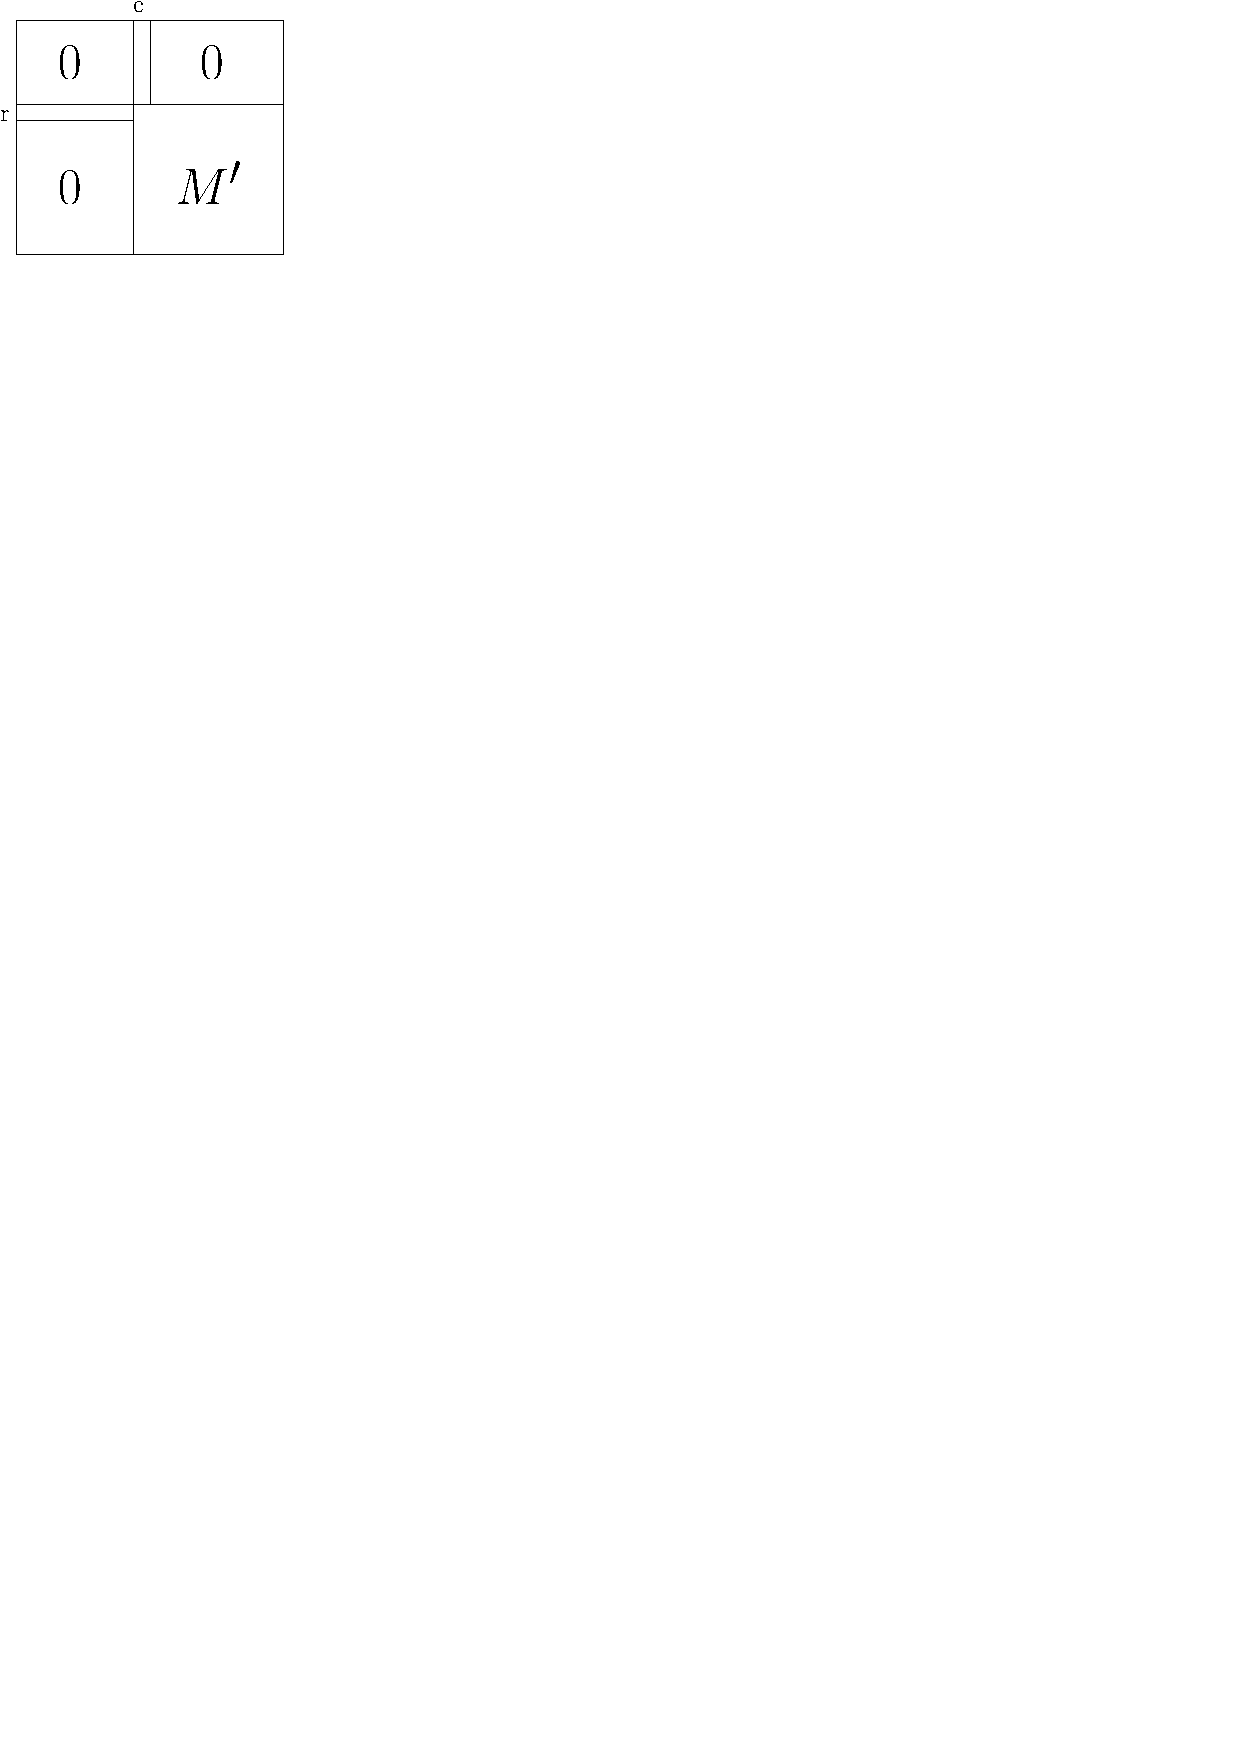
\includegraphics[width=50mm]{img/p12.pdf}
\caption{The characterization of matrices avoiding \usebox{\smlmat} as an interval minor. The matrix $M'$ is a walking matrix.}
\label{fig:p12}
\end{figure}
\begin{proof}
\begin{itemize}
	\item[$\Rightarrow$] If $M$ is a walking matrix then we set $r=c=1$. Otherwise, there are one-entries $M[r,c']$ and $M[r',c]$ such that $r'<r$ and $c'<c$. If an entry~$M[r,c]$ is not top-left, top-right or bottom-left empty then $P_3\im M$. If the submatrix~$M[[r,m],[c,n]]$ is not a walking matrix then it contains $\smm{ &\bullet\\\bullet& }$ and together with the one-entry~$M[r,c']$ it gives us a mapping of $P_3$.
	\item[$\Leftarrow$] For contradiction, assume that a matrix~$M$ described in Figure~\ref{fig:p12} contains $P_3$ as an interval minor. Without loss of generality, let $P_3[1,1]$ be mapped to a one-entry in the $r$-th row. Then both $P_3[1,2]$ and $P_3[2,1]$ need to be mapped to $M'$, which is a contradiction with it being a walking matrix. \qedhere
\end{itemize}
\end{proof}

\pagebreak
\begin{prop}
For all matrices $M$: $P_4\nim M\Leftrightarrow$ there are matrices~$M_1,M_2$ such that  $M=M_1\hsum M_2$, $\smm{\bullet& \\ &\bullet}\nim M_1$ and $\smm{ &\bullet\\\bullet& }\nim M_2$.
\end{prop}
\begin{proof}
\begin{itemize}
	\item[$\Rightarrow$] Let $e=M[r,c]$ be an arbitrary top-most one-entry in $M$. It holds $\smm{\bullet& \\ &\bullet}\nim M[[m],[c-1]]$; otherwise, we have a mapping of $P_4$ to $M$. If we also have $\smm{ &\bullet\\\bullet& }\nim M[[m],[c,n]]$ then we are done. For contradiction, let $e_1,\ e_2$ be any two one-entries forming $\smm{ &\bullet\\\bullet& }$ in $M[[m],[c,n]]$. Symmetrically, let $e'_1,\ e'_2$ be any two one-entries forming $\smm{\bullet& \\ &\bullet}$ in $M[[m],[c]]$. Without loss of generality, let $e_2$ be no higher than $e'_2$ and then, together with $e'_1$ and $e_1$ it gives us a mapping of $P_4$ to $M$, giving a contradiction. 
	\item[$\Leftarrow$] For contradiction, let $P_4\im M$ and consider an arbitrary mapping. Consider the one-entry of $M$, where $P_4[2,2]$ is mapped. If it is in $M_1$ then $\smm{\bullet& \\ &\bullet}\im M_1$ and we get a contradiction. Otherwise, we have $\smm{ &\bullet\\\bullet& }\im M_2$, which is again a contradiction. \qedhere
\end{itemize}
\end{proof}

\begin{prop}
For all matrices $M\in\Mat$: $P_5\nim M\Leftrightarrow$ for every one-entry $M[r,c]$ on the bottom-left extreme walk~$w$, there is at most one non-empty column in $M[[r-1],[c+1,n]]$.
\end{prop}
\begin{proof}
\begin{itemize}
	\item[$\Rightarrow$] For contradiction, assume there is a one-entry~$M[r,c]$ on $w$ such that there are two non-empty columns in $M[[r-1],[c+1,n]]$. Then a one-entry from each of those columns and $M[r,c]$ together give us a mapping of $P_5$ to $M$, and a contradiction. 
	\item[$\Leftarrow$] For contradiction, let $P_5\im M$ and consider any such mapping. Without loss of generality, $P_5[2,1]$ is mapped to a one-entry~$M[r,c]$ from $w$. Then $\smm{\bullet&\bullet}\im M[[r-1],[c+1,n]]$, which is a contradiction with it having one-entries in at most one column. \qedhere
\end{itemize}
\end{proof}

\begin{prop}
For all matrices $M$: $P_6\nim M\Leftrightarrow$ for every one-entry $M[r,c]$ on the bottom-right extreme reverse walk~$w$, $M[[r-1],[c-1]]$ is a walking matrix.
\end{prop}
\begin{proof}
\begin{itemize}
	\item[$\Rightarrow$] For contradiction, assume there are integers~$r,c$ such that $M[r,c]$ is a one-entry on $w$ and $M[[r-1],[c-1]]$ is not a walking matrix. It means that $\smm{ &\bullet\\\bullet& }\im M[[r-1],[c-1]]$ and together with $M[r,c]$ it gives us a mapping of the forbidden pattern, and a contradiction.
	\item[$\Leftarrow$] For contradiction, let $P_6\im M$ and consider an arbitrary mapping of $P_6$. Without loss of generality, let $P_6[3,3]$ be mapped to some one-entry~$M[r,c]$ on $w$. Then, $M[[r],[c]]$ is not a walking matrix and we have a contradiction. \qedhere
\end{itemize}
\end{proof}

\section{Patterns having four one-entries}
\label{sec:4ones}
These are some of the patterns having four one-entries and no empty lines that we did not characterize so far:
$$P_7=\smm{\bullet&\bullet\\\bullet&\bullet}\ \ 
\ P_8=\smm{\bullet&\bullet&\bullet\\ &\bullet& }\ \ 
\ P_9=\smm{\bullet& & & \\ & &\bullet& \\ &\bullet& & \\ & & &\bullet}$$

\begin{lemma}
\label{lemma:p33}
For any matrix $M$: $P_7\nim M\Rightarrow$ there exist integers $r,c$ such that $M[r,c]$ is either
\begin{enumerate}
\item a one-entry and $(r,c)\in\{(1,1),(1,n),(m,1),(m,n)\}$, or
\item top-right and bottom-left empty and $(r,c)\not\in\{(1,1),(m,n)\}$, or
\item top-left and bottom-right empty and $(r,c)\not\in\{(1,n),(m,1)\}$.
\end{enumerate}
\end{lemma}
\begin{proof}
If there is a one-entry in any corner then the first condition is satisfied. Otherwise, consider the entry~$M[2,1]$. It is trivially bottom-left empty and if there is no one-entry in the first row of $M$ then the second condition is satisfied. Therefore, let $M[1,c_t]$ be a one-entry in the first row. Symmetrically, let $M[m,c_b]$ be a one-entry in the last row, let $M[r_l,1]$ be a one-entry in the first column and let $M[r_r,n]$ be a one-entry in the last column.

It cannot at the same time happen that $c_t<c_b$ and $r_r>r_l$ (or symmetrically $c_t>c_b$ and $r_r<r_l$), because then $P_7\im M$. Without loss of generality, let $c_t\geq c_b$ and $r_r\geq r_l$. The submatrix~$M[[r_r-1],[c_t+1,n]]$ is empty; otherwise, any one-entry there, together with $M[1,c_t],M[m,c_b]$ and $M[r_r,1]$ forms the forbidden pattern. Similarly, the matrix $M[[r_r+1,m],[c_t-1]]$ is also empty. Thus $M[r_t,c_t]$ is top-right and bottom-left empty and it is not a corner, satisfying the second condition.
\end{proof}

\begin{prop}
\label{prop:p33}
For all matrices $M\in\Mat$: $P_7\nim M\Leftrightarrow$ there are integers $r,c$ such that either (see Figure~\ref{fig:p33}):
\begin{enumerate}
	\item $M[r,c]$ is top-right empty and bottom-left empty, $\smm{\bullet&\bullet\\\bullet& }\nim M[[r],[c]]$ and $\smm{ &\bullet\\\bullet&\bullet}\nim M[[r,m],[c,n]]$, or
	\item $M[r,c]$ is top-left empty and bottom-right empty, $\smm{\bullet&\bullet\\ &\bullet}\nim M[[r],[c,n]]$ and $\smm{\bullet& \\\bullet&\bullet}\nim M[[r,m],[c]]$.
\end{enumerate}
\end{prop}
\begin{figure}[!ht]
\centering
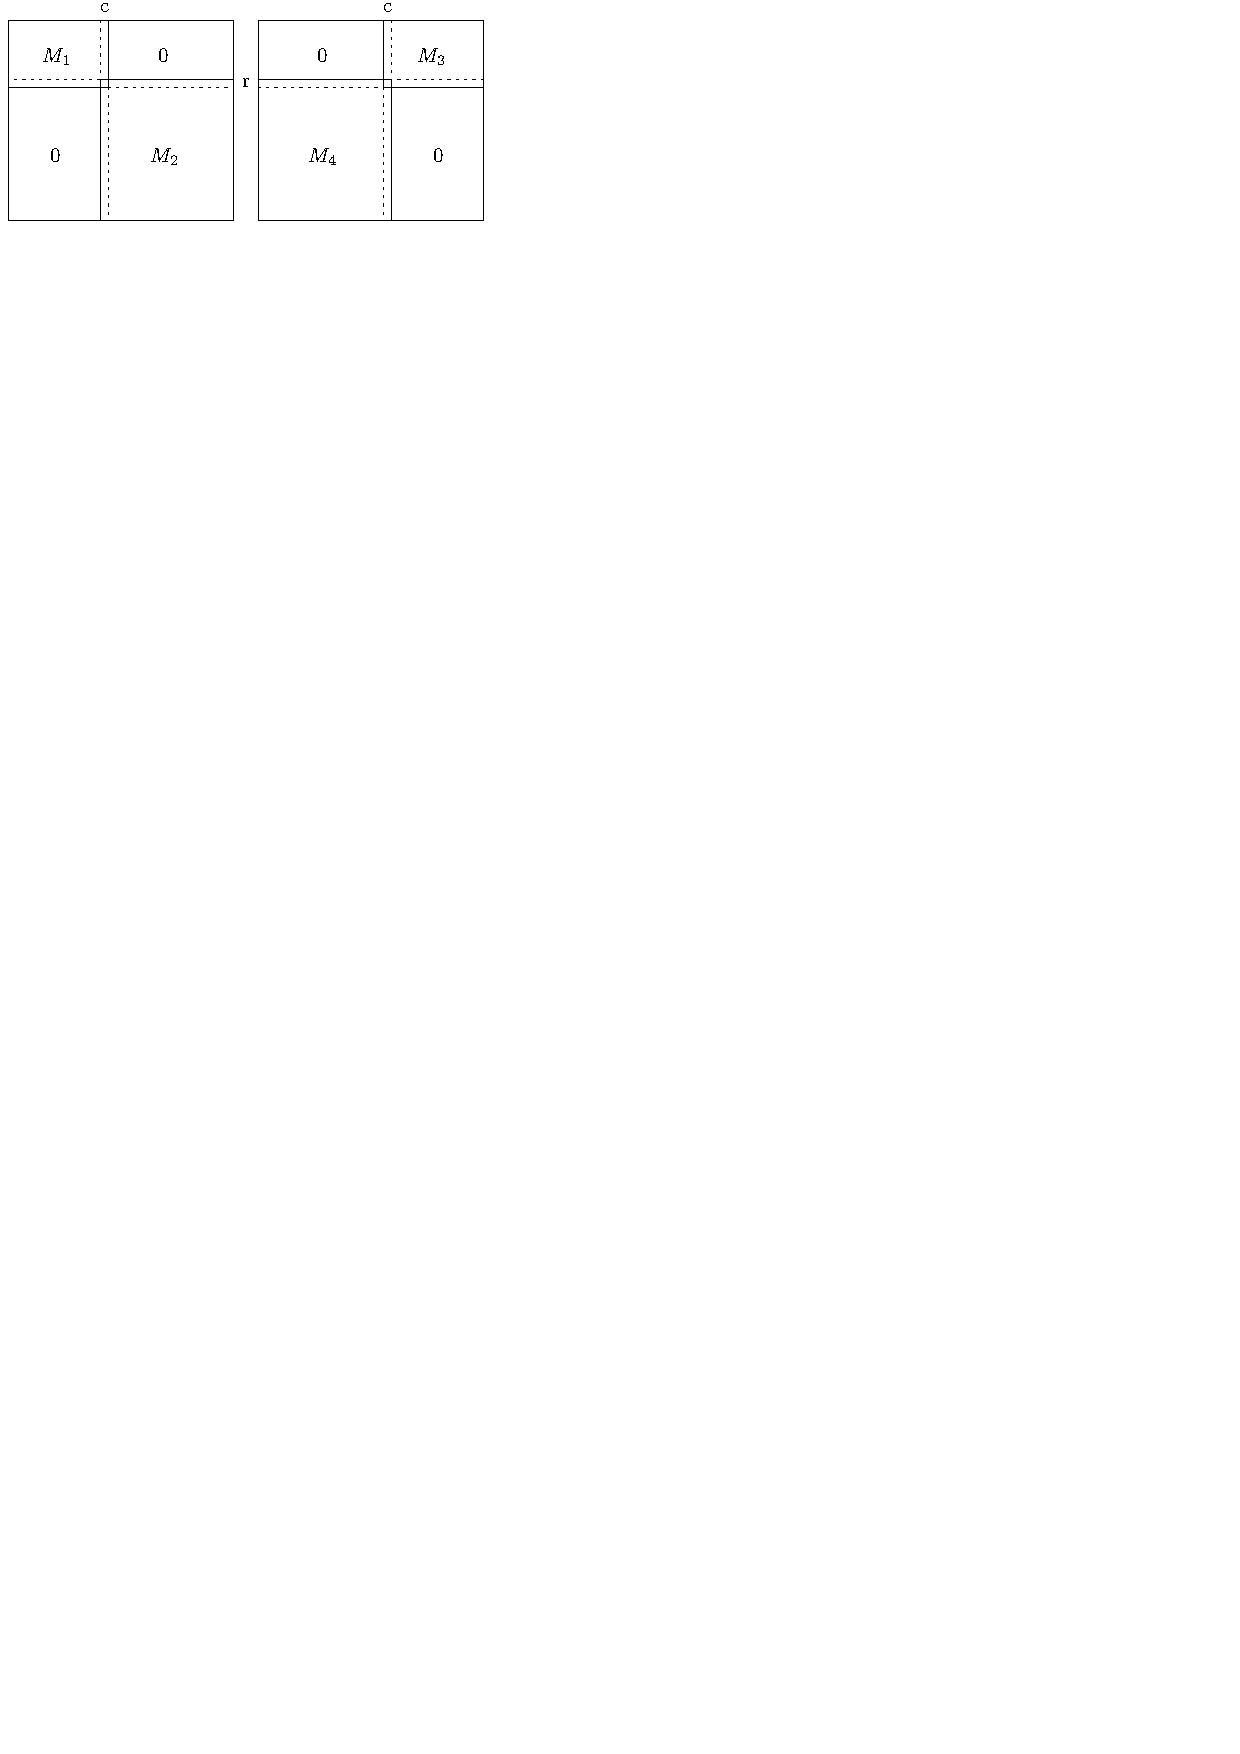
\includegraphics[width=100mm]{img/p33.pdf}
\caption{The characterization of matrices avoiding \usebox{\smlmatb} as an interval minor.}
\label{fig:p33}
\end{figure}
\begin{proof}
We let $M_1=M[[r],[c]],\ M_2=M[[r,m],[c,n]],\ M_3=M[[r],[c,n]]$ and $M_4=M[[r,m],[c]]$.
\begin{itemize}
	\item[$\Rightarrow$] We proceed by induction on the size of $M$.

If $M\in\bin^{2\times2}$ then it either avoids $\smm{ &\bullet\\\bullet&\bullet}$ or $\smm{\bullet&\bullet\\\bullet& }$ and we are done.

For a bigger matrix $M$, from Lemma~\ref{lemma:p33}, there is an entry~$M[r,c]$ satisfying some conditions. If there is a one-entry in any corner, we are done because the matrix cannot contain one of the rotations of $\smm{\bullet&\bullet\\\bullet& }$. Otherwise, assume $M[r,c]$ is both top-right and bottom-left empty and $(r,c)\not\in\{(1,1),(m,n)\}$. If $M_1$ is non-empty, then $\smm{ &\bullet\\\bullet&\bullet}\nim M_2$. Symmetrically, $\smm{\bullet&\bullet\\\bullet& }\nim M_1$ if $M_2$ is non-empty. If one of them is empty, the other is a smaller matrix avoiding $P_7$ as an interval minor and the statement follows from the induction hypothesis.
	\item[$\Leftarrow$] Let $P_7\im M$. Every mapping of $P_7$ partitions $M$ into four non-empty quadrants; thus, there are no integers $r,c$ satisfying the conditions. \qedhere
\end{itemize}
\end{proof}

\begin{lemma}
\label{lemma:p72}
For all matrices $M$: $P_8\nim M\Rightarrow$ there are matrices~$M_1,M_2$ such that $M=M_1\hsum M_2$ and
\begin{enumerate}
\item $\smm{\bullet&\bullet\\ &\bullet}\nim M_1$ and $\smm{ &\bullet\\\bullet& }\nim M_2$, or
\item $\smm{\bullet& \\ &\bullet}\nim M_1$ and $\smm{\bullet&\bullet\\\bullet& }\nim M_2$.
\end{enumerate}
\end{lemma}
\begin{proof}
Let $e=M[r,c]$ be an arbitrary top-most one-entry of the matrix~$M$. It holds $\smm{\bullet&\bullet\\ &\bullet}\nim M[[m],[c-1]]$; otherwise, we have a mapping of $P_8$ to $M$. Symmetrically, $\smm{\bullet&\bullet\\\bullet& }\nim M[[m],[c+1,n]]$. For contradiction with the statement, let $e_1,\ e_2$ (none of them equal to $e$) be any two one-entries forming $\smm{\bullet& \\ &\bullet}$ in $M[[m],[c]]$ and let $e'_1,\ e'_2$ be any two one-entries forming $\smm{ &\bullet\\\bullet& }$ in $M[[m],[c,n]]$. Without loss of generality, $e'_2$ is no higher than $e_2$ and together with $e_1,\ e$ and $e'_1$ it gives us a mapping of $P_8$ to $M$, which is a contradiction.
\end{proof}

\begin{prop}
\label{prop:p72}
For all matrices $M\in\Mat$: $P_8\nim M\Leftrightarrow$ there are integers $r,c_1$ and $c_2$ such that all one-entries of $M$ above the row~$r$ are in columns $c_1$ and $c_2$, $M[[r+1,m],[c_1+1,c_2-1]]$ is empty, $\smm{\bullet& \\ &\bullet}\nim M[[r,m],[c_1]]$ and $\smm{ &\bullet\\\bullet& }\nim M[[r,m],[c_2,n]]$. See Figure~\ref{fig:p72}.
\end{prop}
\begin{figure}[!ht]
\centering
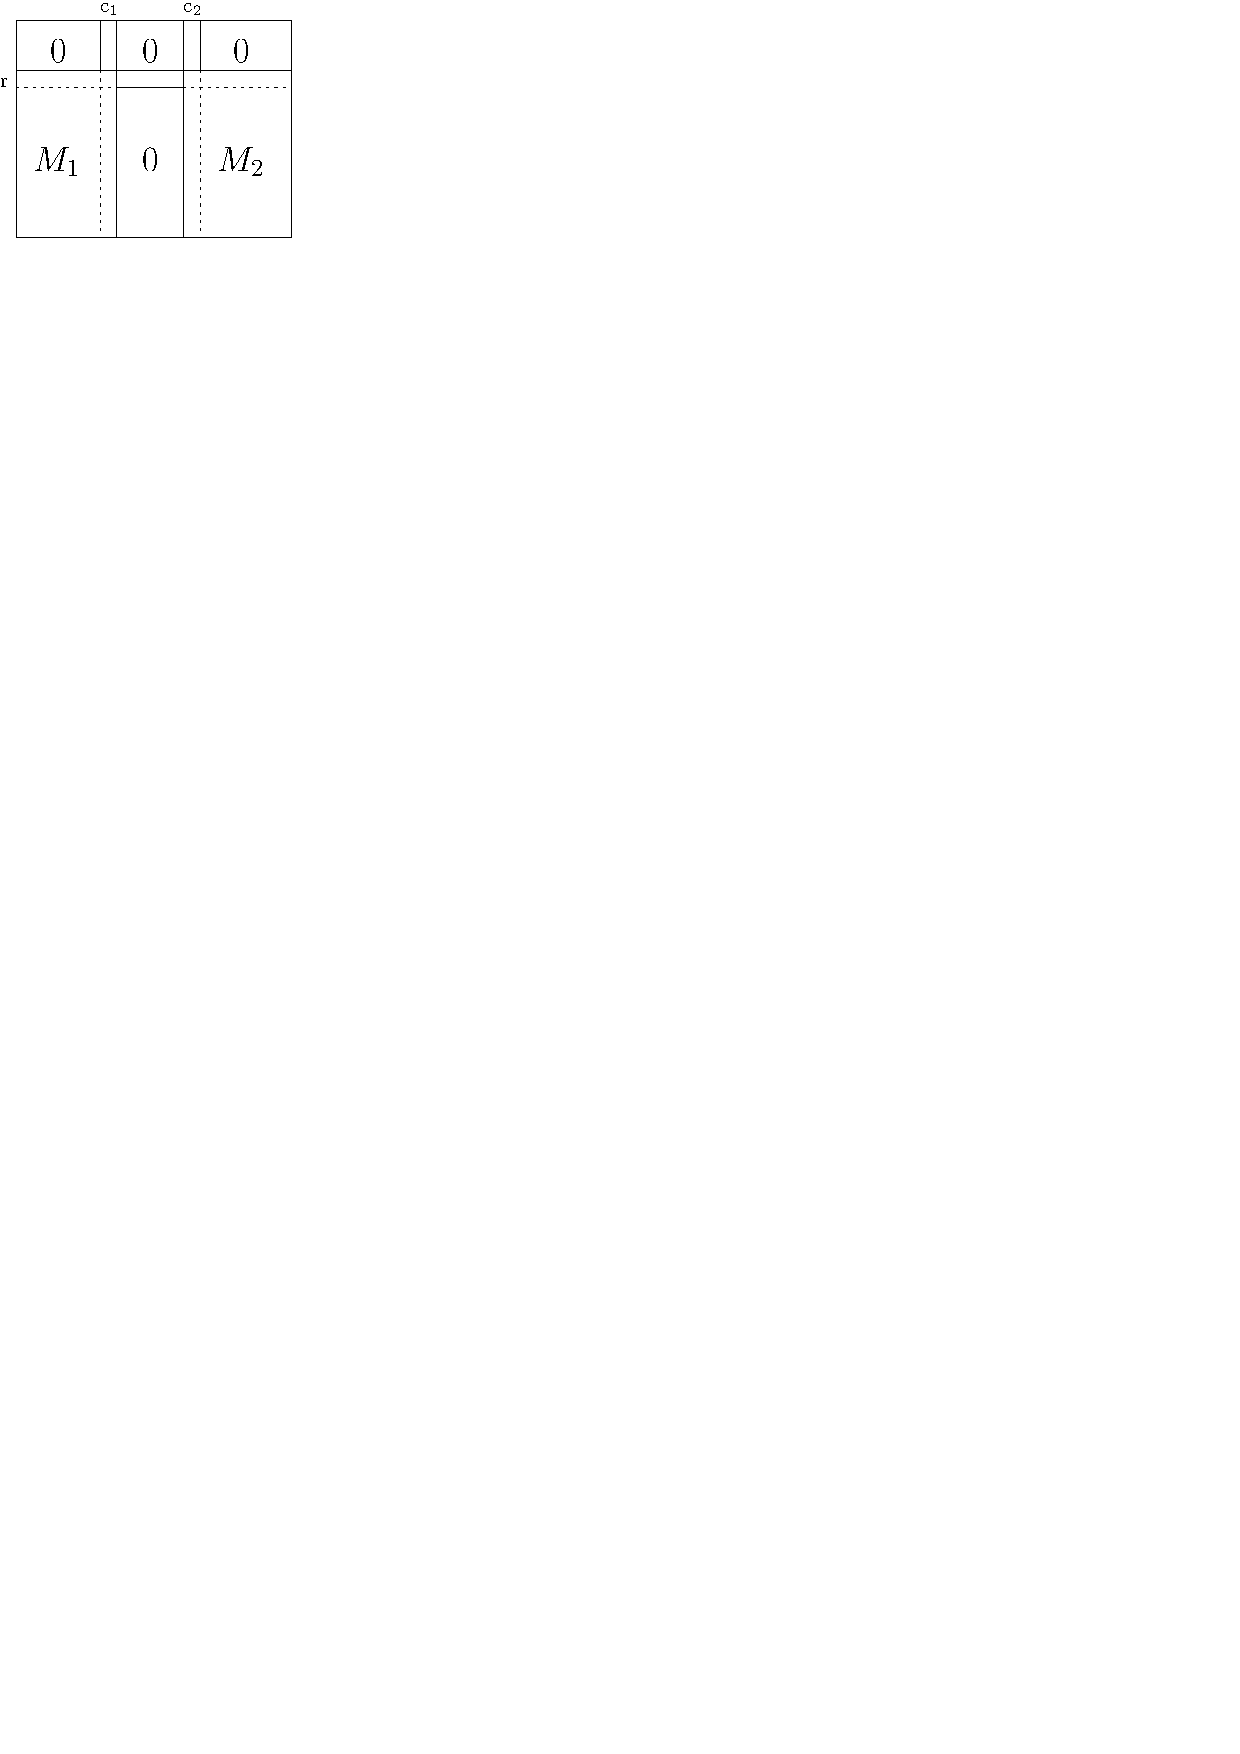
\includegraphics[width=60mm]{img/p72.pdf}
\caption{The characterization of matrices avoiding \usebox{\smlmatc} as an interval minor.}
\label{fig:p72}
\end{figure}
\begin{proof}
\begin{itemize}
	\item[$\Rightarrow$] From Lemma~\ref{lemma:p72}, we know there are matrices~$M_1',M_2'$ such that $M=M_1'\hsum M_2'$, $\smm{\bullet&\bullet\\ &\bullet}\nim M_1'$ and $\smm{ &\bullet\\\bullet& }\nim M_2'$ (or symmetrically the second case). Let $c_2$ be the first column appended from $M_2'$. From Proposition~\ref{prop:p31}, we have integers $r',c'$ such that $M_1'[r',c']$ is top-left, top-right and bottom-right empty and $\smm{\bullet& \\ &\bullet}\im M_1'[[r',m],[c']]=M_1$. Let us set $r=r'$ and $c_1=c'$. We also have that $M[[m],[c_2,n]]$ is a walking matrix. Without loss of generality, $M[[r-1],\{c_1\}]$ and $M[\{r\},[c_1+1,c_2-1]]$ are non-empty; otherwise, we extend $M_1$ to cover the whole $M[[m],[c_2-1]$. There are no two different columns in $M_2'$ having a one-entry above the $r$-th row; otherwise, together with one-entries in $M[[r-1],\{c_1\}]$ and $M[\{r\},[c_1+1,c_2-1]]$ they would give us a mapping of $P_8$ to $M$.
	\item[$\Leftarrow$] A one-entry~$P_8[2,2]$ can not be mapped anywhere but to the $r$-th row, but in that case, there are at most two columns having one-entries above it. \qedhere
\end{itemize}
\end{proof}

\begin{prop}
For all matrices $M\in\Mat$: $P_9\nim M\Leftrightarrow$ for every one-entry~$M[r,c]$ on the bottom-right extreme reverse walk~$w$ and every one-entry~$M[r',c']$ on the top-left extreme reverse walk~$w'$, if $r>r'+3$ and $c>c'+3$ then $M[[r'+1,r-1],[c'+1,c-1]]$ is a walking matrix.
\end{prop}
\begin{proof}
\begin{itemize}
	\item[$\Rightarrow$] If there are one-entries~$M[r,c]$ on $w$ and $M[r',c']$ on $w'$ such that $\smm{ &\bullet\\\bullet& }\im M[[r'+1,r-1],[c'+1,c-1]]$, we have a a mapping of $P_9$ to $M$.
	\item[$\Leftarrow$] For contradiction, let $P_9\im M$ and consider any mapping. Without loss of generality, the one-entry~$P_9[4,4]$ is mapped to some one-entry~$M[r,c]$ on $w$ and the one-entry~$P_9[1,1]$ is mapped to some one-entry~$M[r',c']$ on $w'$. This means that $\smm{ &\bullet\\\bullet& }\im M[[r'+1,r-1],[c'+1,c-1]]$, which is a contradiction with it being a walking matrix. \qedhere
\end{itemize}
\end{proof}

\section{Multiple patterns}
Instead of considering matrices avoiding a single pattern, we can work with matrices avoiding a set of forbidden patterns.

We only describe the structure of matrices avoiding one particular set of patterns, because we use the simple result later.

\begin{prop}
\label{prop:twopatterns}
Let $P_{10}=\smm{\bullet&\circ&\circ\\\circ&\circ&\bullet}$ and $P_{11}=\smm{\bullet&\circ\\\circ&\circ\\\circ&\bullet}$, then for a matrix~$M$: $\{P_{10},P_{11}\}\nim M\Leftrightarrow$ for every $r>1$ and $c>1$, if $M[r,c]$ is a one-entry then it either is on the top-left extreme walk~$w$ or both $M[r-1,c]$ and $M[r,c-1]$ are on $w$.
\end{prop}
\begin{proof}
\begin{itemize}
	\item[$\Rightarrow$] Assume there are $r>1$ and $c>1$ and a one-entry~$M[r,c]$ outside of $w$ such that $M[r-1,c]$ (or $M[r,c-1]$) is outside of $w$. The one-entry~$M[r,c]$ is not top-left extreme and so there is a one-entry in $M'=M[[r-1],[c-1]]$. The entry~$M[r-1,c]$ is not top-left extreme and because $M'$ is non-empty, $M[r-1,c]$ is not top-left empty, and so we have $r>2$. Any one-entry in $M[[r-2],[c-1]]$ together with $M[r,c]$ give us a mapping of $P_{11}$ ($P_{10}$).
	\item[$\Leftarrow$] For any one-entry~$M[r,c]$, there are one-entries in neither $M[[r-2],[c-1]]$ nor $M[[r-1],[c-2]]$. \qedhere
\end{itemize}
\end{proof}